\section{Exploratory analyses}\label{sec:explore}

Everything in this section was computed after the confirmatory run, to understand its outcome. None
of it was pre-registered, and none of it changes a verdict of Table~\ref{tab:verdicts}. The scripts,
logs and result files are in the repository under \texttt{code/exploratory} and
\texttt{exploratory/}.

\subsection{What carries the slow mode}\label{sec:slow}

For the chain on each giant SCC we computed the left and right eigenvectors of $\lambda_2$ and the
sweep cut of smallest conductance along the right eigenvector, a standard way of locating a
metastable set \cite{chung2005,deuflhard2005}: the set $S$ of neurons with the smallest (or
largest) eigenvector entries that minimises
$\phi(S)=F(S\to S^c)/\min\{\pi(S),\pi(S^c)\}$, with $F$ the stationary probability flow per step.

At $w\ge5$ the slow mode is carried by eleven neurons of the VNC (Table~\ref{tab:trap}; VNC type
names follow the systematic nomenclature of the male adult nerve cord connectome
\cite{takemura2024,marin2024,cheong2026}): seven efferent neurons with somata on the midline of the mesothoracic neuromere (EN00B001, EN00B008,
two EN00B011, two EN00B015 and the ventral unpaired median neuron mesVUM-MJ), two IN03B088 and one
IN19A061 interneuron, and one abdominal motor neuron, MNad21. Together they hold 12.8\,\% of the
stationary mass of the chain, a walker leaves them with probability $3.5\times10^{-3}$ per step,
and the two-block estimate $1-p-q=0.99598$ reproduces $\lamtwo=0.99652$. The left eigenvector
puts 99.7\,\% of its negative mass in the cord. The eleven neurons are not a trap at $w\ge1$: there
they hold 0.4\,\% of the stationary mass and a walker leaves them with probability 0.29 per step.
What changes is their output. At $w\ge1$ they send 299 synapses to the other neurons of $G$, only 43 of
them on connections of five or more synapses (six connections), while they receive 21{,}846 synapses,
19{,}378 of them on such connections, and 514 synapses connect them with each other. Dropping weak
connections removes most of the way out and little of the way in. Efferent neurons send their main output out of the CNS, to targets that are not in the
connectome, so the within-CNS normalisation of the chain leaves them with few, mostly local, exits.
This set also sets the certified bound of H3: from $r=4$ on, the witness pair that attains the
bound has one member inside it.

Removing the eleven neurons lowers $\lamtwo$ at $w\ge5$ to 0.9806, and the next metastable set is
again small and in the cord (five VNC interneurons and one motor neuron, 4.0\,\% of the stationary
mass, conductance 0.027). The certified bounds become $0.674\le\Dob(P^{32})\le0.863$ and
$0.107\le\Dob(P^{128})\le0.511$. Removing every efferent superclass instead (24 neurons of the SCC)
gives nearly the same numbers ($\lamtwo=0.9806$, the same six-neuron set next).
At the five-synapse threshold, then, the slowest dynamics of the synapse-flow chain are set by a
succession of small, nearly closed sets in the cord, not by the neck connective
(Figure~\ref{fig:depth}).

\begin{figure}[t]
\centering
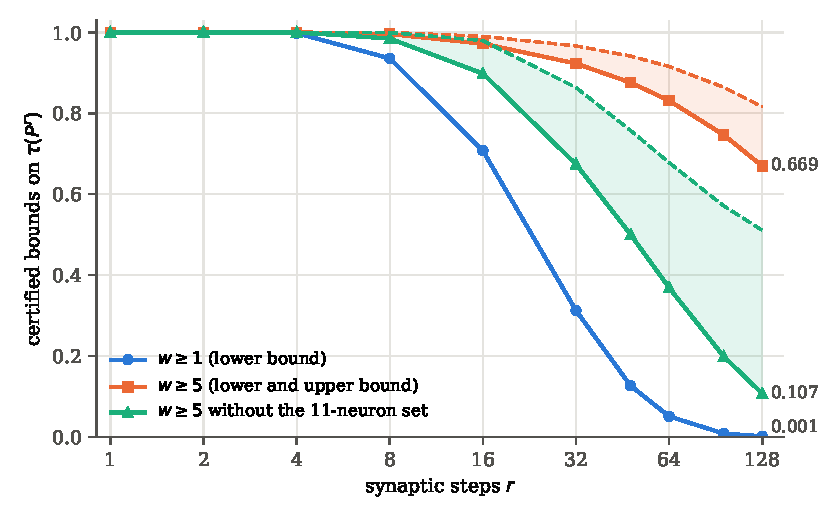
\includegraphics[width=0.82\linewidth]{fig_depth}
\caption{Certified bounds on the Dobrushin coefficient $\Dob(P^r)$ of the synapse-flow chain of the
male CNS: the largest total-variation distance between two starting neurons after $r$ synaptic
steps. Blue: witness lower bound at $w\ge1$ (the nominal chain of H4); orange: lower (solid) and
upper (dashed) bounds at $w\ge5$ (H3); green: the same at $w\ge5$ with the eleven-neuron set of
Table~\ref{tab:trap} removed (exploratory, Section~\ref{sec:slow}). Every bound holds for the exact
chain, with rounding accounted for; the true value lies between the lower and upper curve.}
\label{fig:depth}
\end{figure}

At $w\ge1$ the picture of the exploratory phase holds for the left eigenvector (94.3\,\% of one sign
in the brain, 92.9\,\% of the other in the cord), but no small set dominates: the sweep cut of
smallest conductance is a set of 727 neurons of the central complex and the anterior visual pathway
(414 with primary neuropil in the ellipsoid body; medulla-tubercle, tubercle-bulb, ring, EPG, PEN
and PEG neurons \cite{hulse2021}), with conductance 0.116 and a two-block estimate of 0.883 that does
not reproduce $\lamtwo=0.945$.

\begin{table}[t]
\centering
\small
\caption{The slow mode of the synapse-flow chain. Cut: smallest-conductance sweep set along the slow
right eigenvector; mass: its stationary probability; escape: probability per step that a walker in
the set leaves it (stationary flow divided by mass).}
\label{tab:trap}
\begin{tabular}{@{}lrrrr>{\raggedright\arraybackslash}p{3.8cm}@{}}
\toprule
Chain & $\lamtwo$ & cut size & mass & escape & carried by \\
\midrule
male CNS, $w\ge1$ & 0.94503 & 727 & 0.0047 & 0.116 & central complex, anterior visual pathway \\
male CNS, $w\ge5$ & 0.99652 & 11 & 0.1276 & 0.0035 & mesothoracic efferent neurons \\
male CNS, $w\ge5$, without the 11 & 0.98062 & 6 & 0.0398 & 0.027 & VNC interneurons, one motor neuron \\
FlyWire brain, $w\ge1$ & 0.99999 & 7 & 0.0001 & $2.8\times10^{-5}$ & photoreceptors R1--6, L2 \\
FlyWire brain, $w\ge5$ & 0.95463 & 891 & 0.0177 & 0.069 & anterior visual pathway, central complex \\
male brain only, $w\ge1$ & 0.92559 & 1{,}416 & 0.0179 & 0.114 & anterior visual pathway, central complex \\
male brain only, $w\ge5$ & 0.93179 & 1{,}495 & 0.0150 & 0.105 & anterior visual pathway, central complex \\
\bottomrule
\end{tabular}
\end{table}

\subsection{Is the failure of H4 the certificate or the data?}\label{sec:members}

Lemma~\ref{lem:robust} bounds every chain of the confidence class at once, by a first-order
argument that lets each step take its own worst case. To see how far the depth numbers actually move,
we computed specific chains exactly. $M(c)$ removes every synapse with confidence below $c$, a vertex
of the class at level $c$ (a neuron whose outputs would all be removed keeps them, as the class
allows); $B(k)$ keeps each synapse with probability equal to the midpoint of its confidence bin, a
random reconstruction that is not a member of the class. For each chain we recomputed the distances
$d_r$ of all 4{,}950 pairs of the H4 witness rows and $\lamtwo$ at both thresholds
(Table~\ref{tab:members}).

\begin{table}[t]
\centering
\small
\caption{Chains built from the confidence data (exploratory). $M(c)$: every synapse with confidence
below $c$ removed; $B(k)$: every synapse kept with probability equal to the midpoint of its confidence bin
(five draws).
Synapses: total weight kept; row TV: mean total-variation change of a neuron's output distribution;
set: how many of the eleven neurons of Table~\ref{tab:trap} are in the giant SCC at $w\ge5$;
$\max d_{32}$: the witness lower bound on $\Dob(P'^{32})$ for that chain; $\Delta_{32}$: largest
change of $d_{32}$ over the 4{,}950 witness pairs, relative to $P$.}
\label{tab:members}
\begin{tabular}{@{}lrrrrrrr@{}}
\toprule
Chain & synapses ($10^6$) & row TV & $\lamtwo$, $w\ge1$ & $\lamtwo$, $w\ge5$ & set & $\max d_{32}$ & $\Delta_{32}$ \\
\midrule
\csname @@input\endcsname tab_members_rows.tex
\bottomrule
\end{tabular}
\end{table}

The chains move little (Table~\ref{tab:members}, Figure~\ref{fig:members}). Removing every synapse
below confidence 0.70 changes a neuron's output distribution by 0.080 in total variation on average;
it changes no witness distance at $r=32$ by more than 0.017 (and none at any $r\le64$ by more than
0.043), and $\max d_{32}$ falls from 0.312 to 0.296. Removing every synapse below 0.90, half of all
synapses, lowers $\max d_{32}$ to 0.264. The five random reconstructions remove 15\,\% of the synapses
and change no witness distance at $r=32$ by more than 0.016 (0.11 at $r=8$), while $\max d_r$ moves
by less than 0.01 at every $r$. $M(0.60)$ and $M(0.70)$ are members of the class at $c=0.70$, for
which the certified bound of H4 is negative from $r=8$ on. The second eigenvalue at $w\ge1$ stays
within 0.008 of its value in every chain. At $w\ge5$ it follows the eleven-neuron set of
Section~\ref{sec:slow}. In $M(0.80)$ and $M(0.90)$ the set keeps 15 and none of the 43 synapses on
its connections of five or more synapses to the other neurons of $G$, leaves the giant SCC (one of its
neurons remains in $M(0.80)$), and $\lamtwo$ falls to 0.940 and 0.952. The random reconstructions
keep 21 to 35 of those synapses; where the set stays in the giant SCC with most of its stationary
mass ($B(2)$ and $B(4)$, 8\,\% and 11\,\%) $\lamtwo$ is 0.994 and 0.996, and where it is broken up
(two to six of its neurons left, with mass at most 0.0014) $\lamtwo$ is 0.967 to 0.976, still
above its value at $w\ge1$. The slowest mode at five synapses is thus a property of a few
connections that detection errors can make or break.

\begin{figure}[t]
\centering
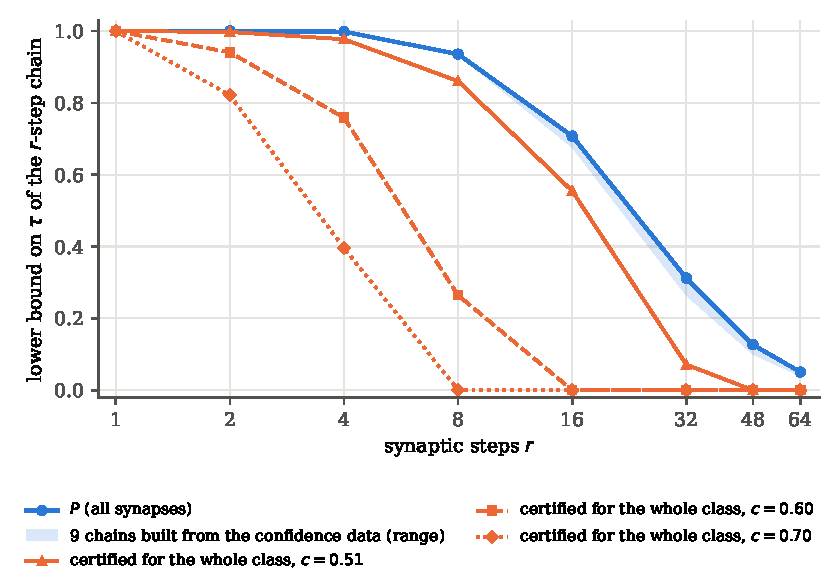
\includegraphics[width=0.82\linewidth]{fig_members}
\caption{The certificate of H4 against exact chains (exploratory). Blue line: witness lower bound
$\max_{a,b}d_r(a,b)$ on $\Dob(P^r)$ for the chain $P$ of all synapses ($w\ge1$, the 4{,}950 pairs of
the H4 witness rows); blue band: its range over the nine chains $M(0.60)$ to $M(0.90)$ and $B(1)$ to
$B(5)$ of Table~\ref{tab:members}. Orange: the certified lower bound of H4
(Lemma~\ref{lem:robust}), valid for every chain of the confidence class at level $c$, drawn at zero
where it is negative, that is, where no certificate is obtained. The chains $M(0.60)$ and $M(0.70)$
belong to the class at $c=0.70$.}
\label{fig:members}
\end{figure}

Where the certificate loses can be located. Lemma~\ref{lem:row} charges row $i$ the fraction
$\varepsilon_i$ of its synapses below the level, which is the largest possible change of the row only
if all of them go to partners that receive no high-confidence synapse from $i$. The exact largest
change over the class has a closed form (proof in Appendix~\ref{app:proofs}).

\begin{lemma}\label{lem:sharp}
For a row with partner weights $w_j$, high-confidence parts $w^{\mathrm{hi}}_j$,
$l_j=w_j-w^{\mathrm{hi}}_j$ and $W=\sum_j w_j$, the largest total-variation change of the normalised
row over the confidence class is
\begin{equation*}
\varepsilon^*=\max_{S}\Bigl[\frac{w(S)}{W}-\frac{w^{\mathrm{hi}}(S)}{W-l(S)}\Bigr]\le\varepsilon,
\end{equation*}
the maximum over nonempty sets $S$ of partners (sums over $S$), attained by removing every
low-confidence synapse to $S$ and none to the other partners. (A row without high-confidence
synapses may be emptied, and then $\varepsilon^*=1$.)
\end{lemma}

We computed $\varepsilon^*$ exactly for rows with at most 12 partners and bounded it from above, still
rigorously, for the others. At $c=0.70$ the mean radius falls from 0.144 to 0.089, close to the 0.080
by which the vertex $M(0.70)$ actually moves a row, but the certificate gains little depth
(Table~\ref{tab:cert}): at $r=4$ the bound rises from 0.396 to 0.621, at $r=8$ it remains negative.
At $c=0.55$ it now certifies $\Dob(P'^{16})\ge0.106$ for the whole class, where the radius of H4 gave
nothing. At $r=32$ the best certificate, at $c=0.51$, rises from 0.071 to 0.096, still short of the
pre-registered 0.10, and from $c=0.52$ on there is none. Most of the slack is in
Lemma~\ref{lem:robust}. Evaluated with the actual row changes
of $M(0.70)$, which is not a certificate but the most favourable radius for that one chain, the lemma
gives $0.026$ at $r=8$, where $M(0.70)$ itself has $0.934$. The lemma adds, at every step, the
perturbations of all the rows that the two walkers visit, as if every one of them pushed the walkers
apart; in the actual chain they point in different directions and largely cancel.

\begin{table}[t]
\centering
\small
\caption{Where the certificate of H4 loses (exploratory). Certified lower bounds on $\Dob(P'^r)$ for
every chain of the confidence class at level $c$, with the row radius of H4 and with the radius of
Lemma~\ref{lem:sharp} (exact for rows with at most 12 partners, a certified upper bound
otherwise); for comparison, Lemma~\ref{lem:robust} evaluated with the actual row changes
of the vertex $M(c)$ (valid for that chain only), and the exact witness bound of $M(c)$ from
Table~\ref{tab:members}. Mean: mean radius over the rows of $G$. A negative value means that no
bound is obtained.}
\label{tab:cert}
\begin{tabular}{@{}llrrrrrr@{}}
\toprule
 & radius & mean & $r=2$ & $r=4$ & $r=8$ & $r=16$ & $r=32$ \\
\midrule
\csname @@input\endcsname tab_cert_rows.tex
\bottomrule
\end{tabular}
\end{table}

\subsection{Null models}\label{sec:null}

Each null model keeps every connection's presynaptic neuron and weight and re-draws its postsynaptic
partner by permuting targets within a group of connections, so out-degrees, out-strengths and the
multiset of in-connections are kept. N1 permutes over all connections; N2 within each pair
(superclass of source, superclass of target); N3 within each pair of cell types (three draws each,
Table~\ref{tab:null}). At $w\ge1$ the configuration null N1 mixes fast ($\lamtwo\approx0.15$, 9\,\%
of the stationary mass on the top 1\,\% of neurons against 42\,\% observed); preserving
superclass-to-superclass counts restores most of the slow mode ($\lamtwo=0.928$), and preserving
type-to-type counts restores all of it ($0.9446$ to $0.9447$ against $0.9450$, with a smallest-conductance cut of
714 to 716 neurons against 727 observed, and 41\,\% of the stationary mass on the top 1\,\%). At $w\ge5$ the superclass
null gives 0.91 to 0.94; the type null reproduces a trap of 11 to 13 neurons in two of three draws
($\lamtwo=0.998$ and $0.996$) and not in the third (0.953). The slow modes are thus a property of
cell-type wiring, and at $w\ge5$ they depend on the particular connections of a few efferent types.

\begin{table}[t]
\centering
\small
\caption{Null models: $\lamtwo$ of the giant SCC (three draws each) and stationary mass of the top
1\,\% of neurons.}
\label{tab:null}
\begin{tabular}{@{}lllll@{}}
\toprule
 & observed & N1 (configuration) & N2 (superclass blocks) & N3 (type blocks) \\
\midrule
$w\ge1$, $\lamtwo$ & 0.945 & 0.155, 0.152, 0.152 & 0.928, 0.928, 0.928 & 0.945, 0.945, 0.945 \\
$w\ge1$, top 1\,\% mass & 0.42 & 0.09 & 0.19 & 0.41 \\
$w\ge5$, $\lamtwo$ & 0.997 & 0.230, 0.224, 0.225 & 0.935, 0.913, 0.913 & 0.998, 0.996, 0.953 \\
$w\ge5$, top 1\,\% mass & 0.73 & 0.13 & 0.27 & 0.72, 0.69, 0.63 \\
\bottomrule
\end{tabular}
\end{table}

\subsection{The FlyWire female brain}\label{sec:flywire}

The same chain on the FlyWire whole-brain connectome of a female fly \cite{dorkenwald2024,schlegel2024}
(version 783, 139{,}255 proofread neurons, 54.5 million synapses \cite{flywire783}) and on the male
CNS with the cord removed (the brain-only row of H1) gives the numbers of Tables~\ref{tab:trap} and
\ref{tab:brains}. Two things agree between the datasets and one does not.

First, the slowest well-populated subsystem is the same in both brains: neurons of the anterior
visual pathway and the central complex \cite{hulse2021}. In FlyWire at $w\ge5$ the cut (891 neurons)
is led by medulla-tubercle (MeTu), tubercle-bulb (TuBu), ring (ER) and EPG neurons and Dm-DRA1; in
the male brain (1{,}416 and 1{,}495 neurons) by MeTu neurons, dorsal-rim R7 photoreceptors, Dm-DRA1
and EPG neurons, with Delta7 neurons at one synapse and Mi15 medulla neurons at five. The conductance of these sets is 0.07 to 0.11. The pathway from the dorsal
rim to the ellipsoid body carries sky-compass information; in the synapse-flow chain it is a weakly
coupled channel. Second, the certified depth profiles are of the same order: the lower bound
on $\Dob(P^{32})$ is 0.28 (FlyWire, $w\ge1$), 0.26 (FlyWire, $w\ge5$), 0.11 and 0.17 (male brain),
against 0.31 for the whole male CNS at $w\ge1$.

What does not agree is $\lamtwo$. In FlyWire at $w\ge1$ it is $0.99999$, set by seven neurons (four
R1--6 photoreceptors, one L2 and two unlabelled optic-lobe neurons) that hold about $10^{-4}$ of the
stationary mass and are left with probability $2.8\times10^{-5}$ per step. Like the efferent
neurons of the male cord, the set sits at an edge of the reconstruction, here the lamina. It
dominates $\lamtwo$ but, carrying almost no stationary mass, has no visible effect on the certified
depth profile. The second eigenvalue of a connectome random walk is a
statement about its most nearly closed set, however small; the depth profile is a statement about
where the walk actually goes.

\begin{table}[t]
\centering
\small
\caption{Brain-only chains: certified lower bounds on $\Dob(P^r)$ (100 witness rows, seed 7) and
the stationary mass of the top 1\,\% of neurons. The whole male CNS at $w\ge1$ is shown for
comparison.}
\label{tab:brains}
\begin{tabular}{@{}lrrrrrr@{}}
\toprule
Chain & neurons & $r=8$ & $r=16$ & $r=32$ & $r=64$ & top 1\,\% mass \\
\midrule
FlyWire brain, $w\ge1$ & 135{,}403 & 0.897 & 0.640 & 0.285 & 0.043 & 0.41 \\
FlyWire brain, $w\ge5$ & 119{,}756 & 0.933 & 0.631 & 0.261 & 0.050 & 0.56 \\
male brain only, $w\ge1$ & 145{,}035 & 0.854 & 0.451 & 0.112 & 0.007 & 0.35 \\
male brain only, $w\ge5$ & 139{,}150 & 0.895 & 0.549 & 0.165 & 0.016 & 0.48 \\
\addlinespace
male CNS, $w\ge1$ & 165{,}314 & 0.936 & 0.707 & 0.312 & 0.051 & 0.42 \\
\bottomrule
\end{tabular}
\end{table}
